\hypertarget{grundzuxfcge-des-urheberrechts}{%
\section{Grundzüge des
Urheberrechts}\label{grundzuxfcge-des-urheberrechts}}

\hypertarget{immaterialguxfcterrecht-geistiges-eigentum}{%
\subsection{Immaterialgüterrecht (Geistiges
Eigentum)}\label{immaterialguxfcterrecht-geistiges-eigentum}}

Schutz vor ungreifbaren Gütern. - Urheberrechte - Designrechte -
Patentrechte - Markenrechte

\begin{figure}
\centering
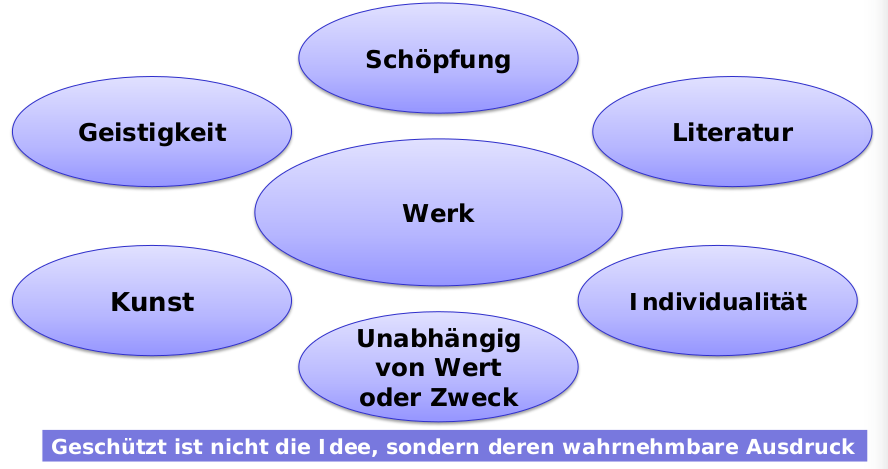
\includegraphics{figures/urheberrechtsSchutz.png}
\caption{Was ist geschützt?}
\end{figure}

\hypertarget{schutzvoraussetzungen}{%
\subsection{Schutzvoraussetzungen}\label{schutzvoraussetzungen}}

\begin{enumerate}
\def\labelenumi{\arabic{enumi}.}
\tightlist
\item
  Literarische, wissenschaftliche und andere Sprachwerke
\item
  Werke der Musik und der bildenden Kunst
\item
  Werke mit wissenschagtlichen oder technischem Inhalt
\item
  Computerprogramme
\item
  Werke der Baukunst
\item
  Fotographische, filmische oder visuelle Werke.
\end{enumerate}

\textbf{Sonderfall: Werke zweiter Hand}\\
Schöpfungen mit individuellem Charakter, die unter Verwendung
bestehender Werke so geschaffen werden, dass die verwendeten Werke in
ihrem individuelle Charakter erkennbar bleiben.

\hypertarget{urheberschaft---miturheberschaft}{%
\subsection{Urheberschaft -
Miturheberschaft}\label{urheberschaft---miturheberschaft}}

\textbf{Urheber} ist die \textbf{natürliche Person}, die das Werk
geschaffen hat (Art. 6 URG) --\textgreater{} \textbf{Schöpferprinzip}.

Eine \textbf{Miturheberschaft} liegt vor, wenn mehrere Personen
gemeinsam, d.h. in \textbf{bewusster Zusammenarbeit} und nach einem
\textbf{gemeinsamen Konzept}, ein Werk schaffen. Dabei steht das
Urheberrecht allen gemeinsam zu (\textbf{Zustimmung aller Miturheber
nötig!})

\hypertarget{abhuxe4ngige-werkschuxf6pfung}{%
\subsection{Abhängige
Werkschöpfung}\label{abhuxe4ngige-werkschuxf6pfung}}

Auch wenn ein Werk \textbf{im Rahmen eines Abhängigkeitsverhältnisses}
geschaffen wird, erwirbt der \textbf{Schöpfer originär} das
\textbf{Urheberrecht}. Nur für \textbf{Computerprogramme} kennt das URG
eine entsprechende Norm (Art. 17 URG). Diese gilt aber auch \textbf{nur}
für den \textbf{Arbeitsvertrag} und nicht für Auftrags- und
Werkvertragsverhältnisse.

Arbeitgeber sollte sich im Arbeitsvertrag sämtliche Urheberrechte
abtreten zu lassen.

\hypertarget{urheberrechte}{%
\subsection{Urheberrechte}\label{urheberrechte}}

\hypertarget{urherberpersuxf6nlichkeitsrechte}{%
\subsubsection{Urherberpersönlichkeitsrechte}\label{urherberpersuxf6nlichkeitsrechte}}

\textbf{Können nicht übertragen werden!}

\begin{itemize}
\tightlist
\item
  Recht auf Erstveröffentlichungen
\item
  Recht auf Anerkennung der Urheberschaft
\item
  Recht auf Werkintegrität
\end{itemize}

\hypertarget{verwendungsrechte}{%
\subsubsection{Verwendungsrechte}\label{verwendungsrechte}}

\textbf{Können übertragen werden! (e.g.~im Arbeitsvertrag)} -
Vervielfältigungsrecht - Verbreitungsrecht - Recht auf öffentliche
Wahrnehmbarmachung - Senderechte - Weitersenderechte - Vermieten von
Computerprogrammen - Bearbeitungsrecht

\hypertarget{schutzvoraussetzungen-und-dauer}{%
\subsection{Schutzvoraussetzungen und
--dauer}\label{schutzvoraussetzungen-und-dauer}}

Der urheberrechtliche Schutz beginnt \textbf{ohne irgendeine Anmeldung}
in dem Moment, in dem ein Werk die Schutzvoraussetzungen erfüllt, d.h.
sobald die Grenze der Individualität überschritten wird (auch Entwürfe
sind geschützt).

Schutzdauer \textbf{70 Jahre nach dem Tod} des Urhebers (\textbf{50
Jahre} bei \textbf{PC-Programmen}). Wenn mehrere Urheber vorhanden sind,
dann beginnt diese Zeit, wenn der letzte ins Grad beisst.

\hypertarget{schranken-des-urheberrechtsschutzes}{%
\subsection{Schranken des
Urheberrechtsschutzes}\label{schranken-des-urheberrechtsschutzes}}

\begin{figure}
\centering
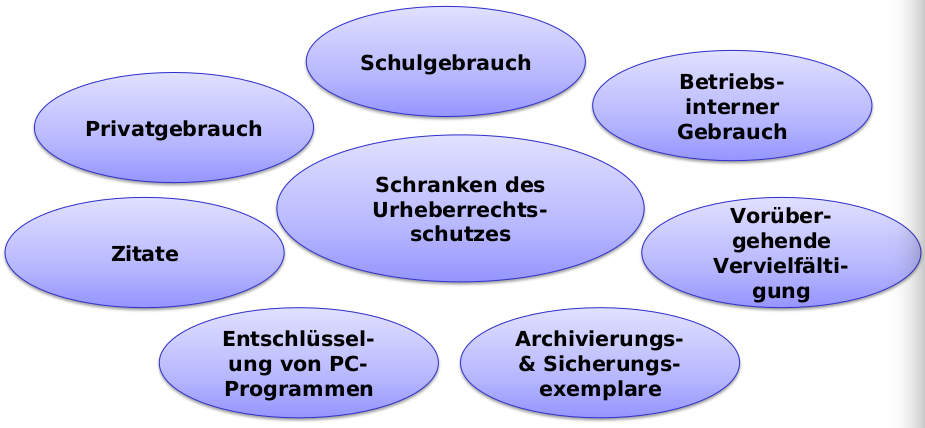
\includegraphics{figures/schrankenUrheberreschtsschutz.png}
\caption{Schranken des Urheberrechtsschutzes}
\end{figure}

\hypertarget{rechtsuxfcbergang-und-rechte-an-programmen}{%
\subsection{Rechtsübergang und Rechte an
Programmen}\label{rechtsuxfcbergang-und-rechte-an-programmen}}

\begin{itemize}
\tightlist
\item
  Die Verwendungsrechte an einem Werk sind unter Lebenden oder
  \textbf{von Todes wegen} vollständig auf Dritte \textbf{übertragbar}
\item
  Die Urheberpersönlichkeitsrechte sind unter Lebenden nicht
  übertragbar, von Todes wegen gehen sie jedoch auf die Erben über
\item
  Als einzige können Computerprogramme als Dienstwerke geschaffen
  werden, sofern der Urheber in einem Arbeitsverhältnis steht und dieses
  zu diesem Zweck (d.h. Schaffung von Computerprogrammen) besteht
\end{itemize}

\hypertarget{rechtsschutz}{%
\subsection{Rechtsschutz}\label{rechtsschutz}}

\textbf{Zivilrechtlicher Schutz} für Schadenersatz und Genugtuung gilt
das Obligationenrecht.

\textbf{Strafrechtlicher Schutz} gilt bei gewerblicher Missachtung des
Urheberrechts. In diesem Fall gibt es Gefängnisstrafen bis zu 3 Jahren.
